\documentclass[12pt]{report}
\usepackage{preamble}

\begin{document}

\title{
  {Constructing Interoperable Blockchains Using NIPoPoWs} \\
  {\large University of Ioannina} \\
}
\author{Kostis Karantias}
\date{\today}

\maketitle

\newpage
\null
\newpage

More detailed title page.

\newpage
\null
\newpage

\begin{abstract}
  In this work we examine the real-world applications of the recent blockchain
  primitive called Non Interactive Proofs of Proof of Work (NIPoPoWs). We
  enable the use of the primitive on Bitcoin Cash by implementing the first
  known velvet fork on a blockchain. We provide concrete implementations for
  creating a velvet fork, and generating proofs on a blockchain that has been
  forked in this way.
\end{abstract}

\newpage

\tableofcontents

\newpage

\thispagestyle{plain}

\chapter{Introduction}

\section{Related Work}
\section{Objectives}
\section{Structure}

\chapter{Background}
\section{Bitcoin}
Bitcoin was introduced in 2008 by Satoshi Nakamoto~\cite{bitcoin} as a
peer-to-peer version of electronic cash, allowing online payments to be sent
directly between parties without the need of a intermediary.

Transfer of value in Bitcoin happens with transactions. A transaction has
inputs and outputs. An output is where the value creation happens for the
receiver. An output can be later redeemed by using its designated receiver's
private key and turned into an input to be used for another transaction.

TODO

\subsection{Block Structure}
A block header contains mainly the hash of the previous block, a Merkle root
hash to commit to a set of transactions, and a nonce.

After the block header comes the series of transactions included in the block.

TODO

\subsection{Proof of Work}
\subsection{Merkle Trees}
A Merkle tree~\cite{merkle} is a data structure which allows a party to
commit to a set of items using only a single hash, and prove the inclusion of
any item in the committed set by providing a logarithmic proof in terms of the
cardinality of the set.

More specifically, the hashes of the items consist the leafs of the tree, and
the last level. The internal levels are defined recursively as follows: To
create level $k-1$ each pair of level $k$ $(A, B)$ is transformed as a node
of value $H(A || B)$ which points to both $A$ and $B$. If the number of nodes
at level $k$ is odd, the last node at that level is paired with itself.
\footnote{This specific construction is the one Bitcoin implements. There are
various other constructions which are not inside the scope of this paper.}

Merkle trees are useful in Bitcoin in order to commit to a set of
transactions to be included in a block while keeping the block header of a
constant size.

To provide proof of inclusion, all a prover has to do is provide a path of
siblings up to the root $\sf{siblings}$ and a bit vector $\sf{left}$ indicating
whether each sibling is on the left or the right. The verification process is
shown in Algorithm~\ref{alg:merkle-verification}.

\begin{algorithm}[H]
  \caption{\label{alg:merkle-verification}The \textsf{Verify} algorithm
    for a Merkle proof}
    \begin{algorithmic}[1]
      \Function{\sf Verify$_{\sf root}$}{\sf leaf, siblings, left}
            \Let{\sf{currentHash}}{\sf{leaf}}
            \While{$\sf{left} \neq []$}
              \Let{\sf{siblingIsLeft}}{\sf{left.shift()}}
              \If{\sf{siblingIsLeft}}
                \Let{\sf{currentHash}}{H(siblings.shift() || currentHash)}
              \Else
                \Let{\sf{currentHash}}{H(currentHash || siblings.shift())}
              \EndIf
            \EndWhile
            \State\Return{currentHash = root}
        \EndFunction
    \end{algorithmic}
\end{algorithm}

An example of a Bitcoin Merkle tree, along with a proof of inclusion for $K$ can be seen on Figure~\ref{fig:merkletree}.

\begin{figure}
  \centering
  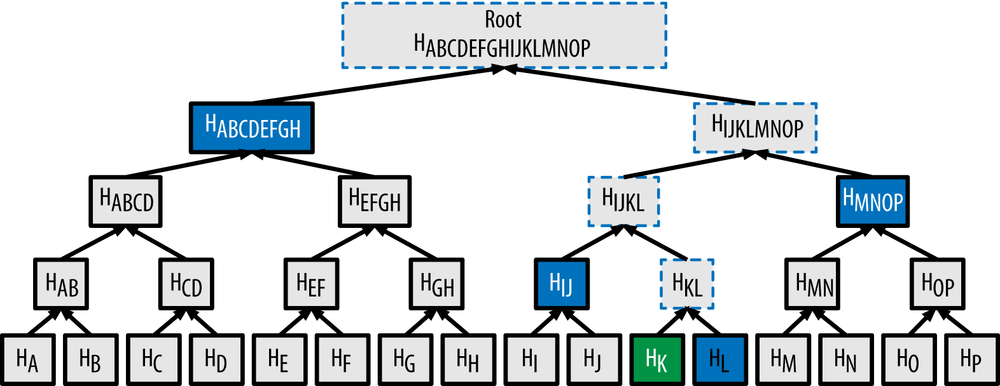
\includegraphics[width=0.9\columnwidth,keepaspectratio]{figures/merkle-tree-proof.png}
  \caption{A Bitcoin Merkle tree. Source:~\cite{mastering}}
  \label{fig:merkletree}
\end{figure}

\subsection{Simplified Payment Verification}
The size of the blockchain has reached 185GB by September 2018, which makes
it a very time consuming or even infeasible process to synchronise a full
node. Fortunately, a solution was proposed in the original whitepaper
~\cite{bitcoin}, which allows the creation of so-called \textit{lite nodes}.
Lite nodes only know the headers of the entire blockchain, which are
constant-size for each block (80 bytes). At the time of writing of this
paper, the size of all block headers was $\sim$42MB. The lite node then asks the
network for transactions concerning it (e.g.\ transactions concerning a
specific public key). Full nodes of the network find such transactions and
return them to the requester. For each transaction, the block header of the
block it's included in is returned, along with a Merkle tree proof of
inclusion which the lite node can then verify. This protocol is reliable as
long as an adversary does not control the network of a lite node.

\subsection{Bitcoin Cash}
In 2017 Bitcoin faced severe scalability issues~\cite{onscaling}. Its limited
1MB block size meant that it could only support a maximum of 7 transactions per
second. As Bitcoin's popularity had exploded at the time, the problem was
hugely exacerbated. The most prominently proposed solution for this was a block
size increase, however no consensus was reached. The discussions ended with a
fork of the main Bitcoin chain which allowed for 8MB blocks, called Bitcoin
Cash.

\section{Non-Interactive Proofs of Proofs of Work}

\subsection{Sublinear SPV}
We would like to be able to prove statements like:

\begin{itemize}
  \item We have a valid chain where the last $k$ blocks are the ones we're
    claiming. This is called a \textbf{suffix proof}.
  \item We have a valid chain where a specific given block is included. This is
    called an \textbf{infix proof}.
\end{itemize}

Our current best solution, SPV, requires providing the whole chain's block
headers as proof. This is obviously linear in the size of the chain.

There have been previous attempts to create proofs smaller in size than SPV
proofs~\cite{KLS}, where a scheme for logarithmic proofs was proposed.
This scheme was later proven insecure~\cite{nipopows}.

NIPoPoWs is the first secure construction~\cite{nipopows} for logarithmic
proofs.

\subsection{Assumptions}
An assumption NIPoPoWs make is that the difficulty is constant. This is not
true for Bitcoin or Bitcoin Cash.

NIPoPoWs also assume each block contains an interlink data structure, which
we'll study shortly. Interlinks too don't exist in Bitcoin or Bitcoin Cash.

In the next section we'll look at how we sidestep all those issues.

\subsection{Levels}
At the heart of the primitive lies the separation of blocks into levels. The
level of a block is defined as $\textit{level}(B) = \left \lfloor \log(T) -
\log(\sf{id}(B)) \right \rfloor$, where $T$ is the constant difficulty of the
blockchain. The genesis block is an exception to this rule as
$\textit{level}(Gen) = \infty$. We call a block of level $\mu$ a $\mu$-superblock.

Intuitively, the level of a block is the number of leading zeros of the binary
representation of the block id when left padded to the length of $T$. An
example of this can be seen on Table~\ref{table:level-counting}.

\begin{table}
  \centering
  \begin{tabular}{|c|c|}
    \hline
    $T$ & 1110000 \\
    \hline
    $\sf{id}(B)$ & \underline{000}1000 \\
    \hline
  \end{tabular}
  \caption{Calculating the level of a block by counting the leading zeros (3 in this case).}
  \label{table:level-counting}
\end{table}

Figure~\ref{fig:hierarchy} shows an example the implied blockchain created from the superblocks.

\begin{figure}
  \centering
  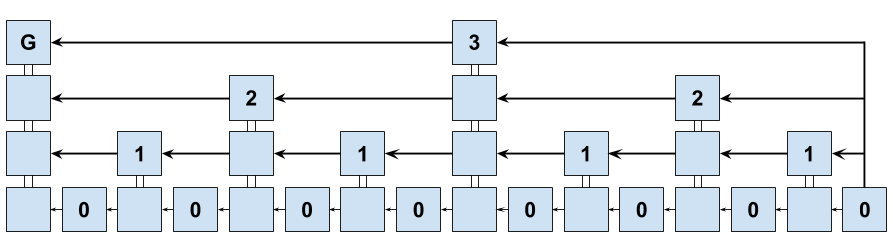
\includegraphics[width=0.9\columnwidth,keepaspectratio]{figures/hierarchical-ledger.png}
  \caption{The hierarchical blockchain.
  Higher levels have achieved a lower target (higher difficulty) during
  mining. All blocks are connected to the genesis block $G$. Source:~\cite{nipopows}}
  \label{fig:hierarchy}
\end{figure}

\subsection{Notation}
The NIPoPoWs paper introduces some notation for talking about blockchains with levels which we'll be using extensively. The notation is widely influenced by Python. Specifically:

\begin{itemize}
  \item $C$ denotes a blockchain, with $C[0]$ being the genesis block, $C[k]$ being the $k$-th first block and $C[-k]$ being the $k$-th last block.
  \item $C[k:]$ denotes the sub-blockchain starting from the $k$-th block, $C[-k:]$ denotes the sub-blockchain starting from the $k$-th last block.
  \item $C[:k]$ denotes the sub-blockchain ending before the $k$-th block, $C[:-k]$ denotes the sub-blockchain ending before the $k$-th last block.
  \item $C[i:j]$ denotes the sub-blockchain starting from the $i$-th block and ending at the $j$-th block. $i$ and $j$ can also be negative numbers similar to above.
  \item $C\upchain^\mu$ denotes the sub-blockset of C where all blocks are of level $\mu$ or higher.
\end{itemize}

\subsection{Interlink}
Instead of keeping only the hash of the previous block inside the block header,
for every superblock level we keep a pointer to the most recent superblock of that level. The structure
containing these pointers is called the interlink. Bitcoin does not support
such a structure in the block header but we will study how to sidestep this
issue by velvet forking in a few sections.

\begin{table}
  \centering
  \begin{tabular}{|c|c|}
    \hline
    Level & Block \\
    \hline
    $0$ & $C[-2]$ \\
    $1$ & $C[-2]$ \\
    $2$ & $C[-4]$ \\
    $3$ & $C[-8]$ \\
    $\infty$ & $C[0]$ \\
    \hline
  \end{tabular}
  \caption{Interlink of $C[-1]$ from Figure~\ref{fig:hierarchy}}
  \label{table:interlink-example}
\end{table}

It's important to note that the interlink can be encoded as a series of block ids, starting from $0$ up to $\infty$. It can also be compressed by using this series as the leafs of a Merkle tree and taking the Merkle tree root.

\subsection{Suffix Proofs}
\subsection{Infix Proofs}
\subsection{Proof Verification}
\subsection{Velvet Forks}
Velvet forks~\cite{nipopows,velvet} describe a formalization of adding
arbitrary data inside blocks in order to allow potential applications without
sacrificing the backwards compatibility of the blockchain. TODO

\subsection{User-Activated Velvet Forks}


\chapter{Bitcoin Cash Velvet Fork Implementation}

\section{Bitcoin-ABC}
\section{Interlinker}

\chapter{NIPoPoW Velvet Fork Prover Implementation}

\section{bcash}
\section{Testing}

\chapter{Results \& Future Work}

\bibliography{bibliography}

\end{document}
